              %******************************************%
              %                                          %
              %     Modello di articolo scientifico      %
              %            di Lorenzo Pantieri ©         %
              %                                          %
              %                © 2013-2017               %
              %                                          %
              %******************************************%
       
% I seguenti commenti speciali impostano:
% 1. utf8 come codifica di input,
% 2. PDFLaTeX come motore di composizione;
% 3. Articolo.tex come documento principale;
% 4. il controllo ortografico italiano per l'editor.

% !TEX encoding = UTF-8 Unicode
% !TEX TS-program = pdflatex
% !TEX root = Articolo.tex
% !TEX spellcheck = it-IT

\documentclass[11pt,%                       % corpo del font principale
               a4paper,%                    % carta A4
               oneside,%                    % solo fronte
%              twoside,%                    % fronte-retro
               headinclude,footinclude,%    % testatina e piede di pagina
               BCOR5mm,%                    % rilegatura di 5 mm
               captions=tableheading,%      % didascalie in cima alle tabelle
               ]{scrartcl}                  % classe report di KOMA-Script;
               
\usepackage[T1]{fontenc}                    % codifica dei font:
                                            % NOTA BENE! richiede una distribuzione *completa* di LaTeX,
                                            % per esempio TeXLive o MiKTeX *complete*

\usepackage[utf8]{inputenc}                 % codifica di input; anche [latin1] va bene
                                            % NOTA BENE! va accordata con le preferenze dell'editor

\usepackage[english,italian]{babel}         % per scrivere in italiano e in inglese;
                                            % l'ultima lingua (l'italiano) risulta predefinita

\usepackage{indentfirst}                    % rientra il primo capoverso di ogni sezione

\usepackage{graphicx}                       % immagini

\usepackage{listings}                       % codici

\usepackage[font=small]{quoting}            % citazioni

\usepackage{amsmath,amssymb,amsthm}         % matematica

\usepackage[italian]{varioref}              % riferimenti completi della pagina
 
\usepackage{tabularx}                       % tabelle di larghezza prefissata

\usepackage[style=philosophy-modern,hyperref,square]{biblatex}
                                            % eccellente pacchetto per la bibliografia;
                                            % produce uno stile di citazione autore-anno; 
                                            % lo stile "numeric-comp" produce riferimenti numerici
                                          
\addbibresource{Bibliografia.bib}           % database di biblatex 
                                          
\usepackage{subfig}                         % sottofigure, sottotabelle

\usepackage{lipsum}                         % testo fittizio

\usepackage{eurosym}                        % simbolo dell'euro

\usepackage[nochapters,%                    % per scrivere un articolo        
            subfig,%                        % se si usa il pacchetto subfig
            beramono,%                      % Bera Mono come font a spaziatura fissa
            eulermath,%                     % AMS Euler come font per la matematica
            pdfspacing,%                    % migliora il riempimento di riga
            listings,%                      % codici
%           parts,%                         % da decommentare in un articolo diviso in parti
            ]{classicthesis}                % stile ClassicThesis

\usepackage{arsclassica}                    % modifica alcuni aspetti di ClassicThesis

%*********************************************************************************
% impostazioni-articolo.tex
% di Lorenzo Pantieri (2013-2016)
% file che contiene le impostazioni dell'articolo
%*********************************************************************************


%*********************************************************************************
% Comandi personali
%*******************************************************
\newcommand{\myName}{Marco De Martino}                            % autore
\newcommand{\myTitle}{Appunti sul marmo}  % titolo
\newcommand{\mySubtitle}{Studio sulla memoria acustica di \newline San Luca e Martina}
\date{}                                                           % nessuna data

\title{\normalfont\spacedallcaps{\myTitle}}
\subtitle{\bigskip~~~~~\normalfont\spacedallcaps{\mySubtitle}}
\author{\spacedlowsmallcaps{\myName}}



%*********************************************************************************
% Impostazioni di amsmath, amssymb, amsthm
%*********************************************************************************

% comandi per gli insiemi numerici (serve il pacchetto amssymb)
\newcommand{\numberset}{\mathbb}
\newcommand{\N}{\numberset{N}}
\newcommand{\R}{\numberset{R}}

% un ambiente per i sistemi
\newenvironment{sistema}%
  {\left\lbrace\begin{array}{@{}l@{}}}%
  {\end{array}\right.}

% definizioni (serve il pacchetto amsthm)
\theoremstyle{definition}
\newtheorem{definizione}{Definizione}

% teoremi, leggi e decreti (serve il pacchetto amsthm)
\theoremstyle{plain}
\newtheorem{teorema}{Teorema}
\newtheorem{legge}{Legge}
\newtheorem{decreto}[legge]{Decreto}
\newtheorem{murphy}{Murphy}[section]



%*********************************************************************************
% Impostazioni di biblatex
%*********************************************************************************
\defbibheading{bibliography}{%
\manualmark
\phantomsection
\addcontentsline{toc}{section}{\refname}
\section*{\bibname\markboth{\spacedlowsmallcaps{\refname}}
{\spacedlowsmallcaps{\refname}}}}



%*********************************************************************************
% Impostazioni di listings
%*********************************************************************************
\lstset{language=[LaTeX]Tex,%C++,
    keywordstyle=\color{RoyalBlue},%\bfseries,
    basicstyle=\small\ttfamily,
    %identifierstyle=\color{NavyBlue},
    commentstyle=\color{Green}\ttfamily,
    stringstyle=\rmfamily,
    numbers=none,%left,%
    numberstyle=\scriptsize,%\tiny
    stepnumber=5,
    numbersep=8pt,
    showstringspaces=false,
    breaklines=true,
    frameround=ftff,
    frame=single
}



%*********************************************************************************
% Impostazioni di hyperref (decommenta le seguenti righe se non carichi arsclassica)
%*********************************************************************************
%\hypersetup{%
%    hyperfootnotes=false,pdfpagelabels,
%    %draft,	% = elimina tutti i link (utile per stampe in bianco e nero)
%    colorlinks=true, linktocpage=true, pdfstartpage=1, pdfstartview=FitV,%
%    % decommenta la riga seguente per avere link in nero (per esempio per la stampa in bianco e nero)
%    %colorlinks=false, linktocpage=false, pdfborder={0 0 0}, pdfstartpage=1, pdfstartview=FitV,%
%    breaklinks=true, pdfpagemode=UseNone, pageanchor=true, pdfpagemode=UseOutlines,%
%    plainpages=false, bookmarksnumbered, bookmarksopen=true, bookmarksopenlevel=1,%
%    hypertexnames=true, pdfhighlight=/O,%nesting=true,%frenchlinks,%
%    urlcolor=webbrown, linkcolor=RoyalBlue, citecolor=webgreen, %pagecolor=RoyalBlue,%
%    %urlcolor=Black, linkcolor=Black, citecolor=Black, %pagecolor=Black,%
%    pdftitle={\myTitle},%
%    pdfauthor={\textcopyright\ \myName},%
%    pdfsubject={},%
%    pdfkeywords={},%
%    pdfcreator={pdfLaTeX},%
%    pdfproducer={LaTeX with hyperref and ClassicThesis}%
%}



%*********************************************************************************
% Impostazioni di graphicx
%*********************************************************************************
\graphicspath{{Immagini/}} % cartella dove sono riposte le immagini



%*********************************************************************************
% Altro
%*********************************************************************************

% [...] ;-)
\newcommand{\omissis}{[\dots\negthinspace]}

% eccezioni all'algoritmo di sillabazione
\hyphenation{Fortran ma-cro-istru-zio-ne nitro-idrossil-amminico}



\areaset[current]{370pt}{750pt}
\setlength{\marginparwidth}{7em}
\setlength{\marginparsep}{2em}%
               % file con le impostazioni personali

\begin{document}
\pagestyle{scrheadings} 
%******************************************************************
% Materiale iniziale
%******************************************************************
% !TEX encoding = UTF-8
% !TEX TS-program = pdflatex
% !TEX root = ../Tesi.tex
% !TEX spellcheck = it-IT

%*******************************************************
% Frontespizio
%*******************************************************
\begin{frontespizio}
\Preambolo{\usepackage{iwona}} % riga da commentare se non si carica ArsClassica

\Universita{Conservatorio di Musica S. Cecilia di Roma}
\Logo{Sigillo}
\Facolta{Dipartimento di Nuove Tecnologie}
\Corso{Musica Elettronica}
\Annoaccademico{2015--2016}
\Titoletto{TRIENNIO DI I LIVELLO}
\Titolo{appunti sul marmo}
\Sottotitolo{sottotitolo}
\Candidato[2240TR]{Marco De Martino}
\Relatore{Giuseppe Silvi}
%\Relatore{Claudio Beccari}
%\Correlatore{Tommaso Gordini}
%\Correlatore{Ivan Valbusa}
\end{frontespizio}
% !TEX encoding = UTF-8
% !TEX TS-program = pdflatex
% !TEX root = ../CME-III-ARTICOLO.tex
% !TEX spellcheck = it-IT

%*******************************************************
% Indici
%*******************************************************
\pdfbookmark{\contentsname}{tableofcontents}
\setcounter{tocdepth}{2}
\tableofcontents
\markboth{\spacedlowsmallcaps{\contentsname}}{\spacedlowsmallcaps{\contentsname}} 

%*******************************************************
% Elenco delle figure
%*******************************************************    
\phantomsection
\pdfbookmark{\listfigurename}{lof}
\listoffigures

%*******************************************************
% Elenco delle tabelle
%*******************************************************
\phantomsection
\pdfbookmark{\listtablename}{lot}
\listoftables
        

% !TEX encoding = UTF-8
% !TEX TS-program = pdflatex
% !TEX root = ../Articolo.tex
% !TEX spellcheck = it-IT

%*******************************************************
% Sommario+Abstract
%*******************************************************
\phantomsection
\pdfbookmark{Sommario}{Sommario}
\section*{Sommario}

\lipsum[1]

\selectlanguage{english}
\pdfbookmark{Abstract}{Abstract}
\section*{Abstract}

\lipsum[2]

\selectlanguage{italian}


%******************************************************************
% Materiale principale
%******************************************************************
% !TEX encoding = UTF-8
% !TEX TS-program = pdflatex
% !TEX root = ../Articolo.tex
% !TEX spellcheck = it-IT

%************************************************
\section{Lorem}
\label{sec:lorem}
%************************************************

\begin{figure}
\centering
\subfloat[Asia personas duo]
{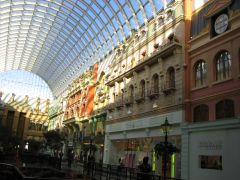
\includegraphics[width=.45\columnwidth]{Lorem}} \quad
\subfloat[Pan ma signo]
{\label{fig:example-b}%
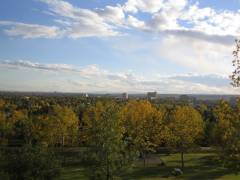
\includegraphics[width=.45\columnwidth]{Ipsum}} \\
\subfloat[Methodicamente o uno]
{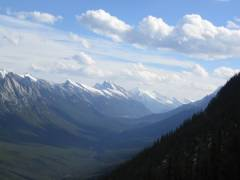
\includegraphics[width=.45\columnwidth]{Dolor}} \quad
\subfloat[Titulo debitas]
{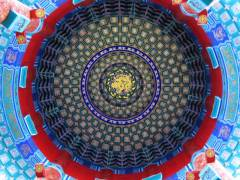
\includegraphics[width=.45\columnwidth]{Sit}}
\caption[Tu duo titulo debitas latente]{Tu duo titulo debitas latente}
\label{fig:example}
\end{figure}

Please note that the content of this section is just some dummy text. It isn't a real language.

Lorem ipsum dolor sit amet, consectetuer adipiscing elit. Ut purus elit, vestibulum ut, placerat ac, adipiscing vitae, felis. Curabitur dictum gravida mauris.

\subsection*{A subsection}

\lipsum[2]

\subsubsection*{A sub-subsection}

\lipsum[7]

\paragraph{A paragraph}
Lorem ipsum dolor sit amet, consectetuer adipiscing elit. Ut purus elit, vestibulum ut, placerat ac, adipiscing vitae, felis. Curabitur dictum gravida mauris. Nam arcu libero, nonummy eget, consectetuer id, vulputate a, magna.

\paragraph{Another paragraph}
Cras nec ante, pellentesque a nulla, cum sociis natoque penatibus et magnis dis parturient montes, nascetur ridiculus mus. Aliquam tincidunt urna

\bigskip

Donec aliquet, tortor sed accumsan bibendum, erat ligula aliquet magna, vitae ornare odio metus a mi. Morbi ac orci et nisl hendrerit mollis. Suspendisse ut massa. Cras nec ante. Pellentesque a nulla. Cum sociis natoque penatibus et magnis dis parturient montes, nascetur ridiculus mus. Aliquam tincidunt urna.

\begin{description}
\item[Mane] Lorem ipsum dolor sit amet, consectetuer adipiscing elit. 
\item[Tekel] Ut purus elit, vestibulum ut, placerat ac, adipiscing vitae, felis. Curabitur dictum gravida mauris.
\item[Fares] Nam arcu libero, nonummy eget, consectetuer 
id, vulputate a, magna.
\end{description}

\begin{table}
\caption{Lorem ipsum dolor sit amet}
\centering
\begin{tabular}{ll}
\toprule
\textbf{Alkaloid} & \textbf{Origin} \\
\midrule
atropine & belladonna \\
morphine & poppy \\
nicotine & tobacco \\
\bottomrule
\end{tabular}
\end{table}

Suspendisse vel felis. Ut lorem lorem, interdum eu, tincidunt sit amet, laoreet vitae, arcu. Aenean faucibus pede eu ante. Praesent enim elit, rutrum at, molestie non, nonummy vel, nisl. Ut lectus eros, malesuada sit amet, fermentum eu, sodales cursus, magna. Donec eu purus. Quisque vehicula, urna sed ultricies auctor, pede lorem egestas dui, et convallis elit erat sed nulla.

\subsection*{Some formulas}

Una formula in linea viene incorporata nel testo: $\lim_{n \to \infty}\sum_{k=1}^n \frac{1}{k^2} = \frac{\pi^2}{6}$, per esempio. Come si osserva, \LaTeX{} fa \emph{il possibile} per comprimerla e modificare il meno possibile l'interlinea nel capoverso che la contiene.
Una formula in display viene invece composta da \LaTeX{} su linee a parte, separate dal contesto con adeguati spazi bianchi per metterla in mostra e farla risaltare sulla pagina.
\begin{equation}
\lim_{n \to \infty}\sum_{k=1}^n \frac{1}{k^2}= \frac{\pi^2}{6}
\end{equation}
Come si osserva, ora la formula risulta centrata, non compressa, e tutti i suoi elementi occupano il giusto spazio con un risultato finale di grande respiro.

Integer tempus convallis augue. Etiam facilisis. Nunc elementum fermentum wisi. Aenean placerat. Ut imperdiet, enim sed gravida sollicitudin, felis odio placerat quam, ac pulvinar elit purus eget enim. 

\begin{equation}
\int_a^{a+T}f(x)\,dx= \int_0^T f(x)\,dx 
\qquad
\oint f(z)\,dz=2\pi i
\end{equation}

Nulla malesuada porttitor diam. Donec felis erat, congue non, volutpat at, tincidunt tristique, libero. Vivamus viverra fermentum felis. Donec non- ummy pellentesque ante.

\begin{equation}
f(x_1,\dots,x_n)=  \prod_{k=1}^n x_k 
\qquad
\sum_{k=1}^n x_k^2=1
\qquad
\biggl(\sum_n x_n^2\biggr)^{1/2} 
\end{equation}

\lipsum[2]

\begin{equation}
\begin{bmatrix} 
a_{11} & \dots & a_{1n} \\ 
a_{21} & \dots & a_{2n} \\ 
\hdotsfor{3} \\ 
a_{n1} & \dots & a_{nn} 
\end{bmatrix}
\end{equation}

\lipsum[4]

\begin{equation}
\lim_{x\to 0}
\frac{\sin x}{x}=1 \qquad
\lim_{n\to +\infty}f_n=\delta
\end{equation}

Fusce mauris. Vestibulum luctus nibh at lectus. Sed bibendum, nulla a faucibus semper, leo velit ultricies tellus, ac venenatis arcu wisi vel nisl. Vestibulum diam.

\begin{equation}
n!=
\begin{cases} 
1       & \text{if $n=0$} \\ 
n(n-1)! & \text{if $n\ge 1$} 
\end{cases} 
\end{equation}

Ut lectus eros, malesuada sit amet, fermentum eu, sodales cursus, magna. Donec eu purus. Quisque vehicula, urna sed ultricies auctor, pede lorem egestas dui, et convallis elit erat sed nulla. Donec luctus. Curabitur et nunc. Aliquam dolor odio, commodo pretium, ultricies non, pharetra in, velit.

\begin{equation} 
x_G=
\frac{\displaystyle
      \sum_{i=1}^n m_ix_i}
{\displaystyle\sum_{i=1}^n m_i}
\end{equation}

\lipsum[6]

\begin{equation}
\kappa =\frac{\xi}{E_{\textrm{max}}}
\qquad
E_{\textup{max}} =\frac{2 m_{\textup{e}} \beta^2\gamma^2 }{1 +2\gamma m_{\textup{e}}/m_{\textrm{x}} + ( m_{\textup{e}}/m_{\textup{x}})^2}
\end{equation}

\lipsum[8]
% !TEX encoding = UTF-8
% !TEX TS-program = pdflatex
% !TEX root = ../Tesi.tex
% !TEX spellcheck = it-IT

%************************************************
\chapter{Ipsum}
\label{cap:ipsum}
%************************************************

\lipsum[1]

\section{Lorem}
\lipsum[2]

\section{Ipsum}
\lipsum[3]

\section{Dolor}
\lipsum[4-5]
\appendix
% !TEX encoding = UTF-8
% !TEX TS-program = pdflatex
% !TEX root = ../Articolo.tex
% !TEX spellcheck = it-IT

%************************************************
\section{Dolor}
\label{sec:dolor}
%************************************************

\lipsum[1]

\subsection{Mane}
\lipsum[2]

\subsection{Tekel}
\lipsum[3]

\subsection{Fares}
\lipsum[4-5]

% *****************************************************************
% Materiale finale
%******************************************************************
% !TEX encoding = UTF-8
% !TEX TS-program = pdflatex
% !TEX root = ../CME-III-ARTICOLO.tex
% !TEX spellcheck = it-IT

%*******************************************************
% Bibliografia
%*******************************************************
\nocite{*}
\printbibliography
\end{document}